\subsubsection{Introduction d'un déphasage}
Si maintenant, on modifie les phase \lstinline{phi0} et \lstinline{phi1} du Code \ref{code:syn-ideal} de la manière suivante :
\begin{lstlisting}[caption=Introduction d'un déphasage]
phi0 = rand * 2 * pi;
phi1 = rand * 2 * pi;
\end{lstlisting}
on trouve alors un taux d'erreur aléatoire, non nul.
En effet, si nous reprenons les calculs précédents, on a maintenant :
\[
   \left\{
   \begin{array}{rcl}
      I_{0, 0} & = & \int_{0}^{T_s}  cos( 2 \pi F_0 t + \phi_0 )(cos(2\pi F_0t+\phi_0') dt \\
      I_{0, 1} & = & \int_{0}^{T_s}  cos( 2 \pi F_0 t + \phi_0 )(cos(2\pi F_0t+\phi_1') dt \\
      I_{1, 0} & = & \int_{0}^{T_s}  cos( 2 \pi F_0 t + \phi_1 )(cos(2\pi F_0t+\phi_0') dt \\
      I_{1, 1} & = & \int_{0}^{T_s}  cos( 2 \pi F_0 t + \phi_1 )(cos(2\pi F_0t+\phi_1') dt \\
   \end{array}
   \right.
\]
On se retrouve alors avec du $\frac{T_s}{2}cos(\phi_0-\phi_0')$. Selon le déphasage, cette quantité peut être positive ou négative. Ainsi le signe du résultat ne dépend plus que du bit initial, mais aussi de cette erreur aléatoire.
Le récepteur ne fonctionne plus.
\subsubsection{Présentation d'un nouveau récepteur}

\begin{figure}[H]
   \centering
   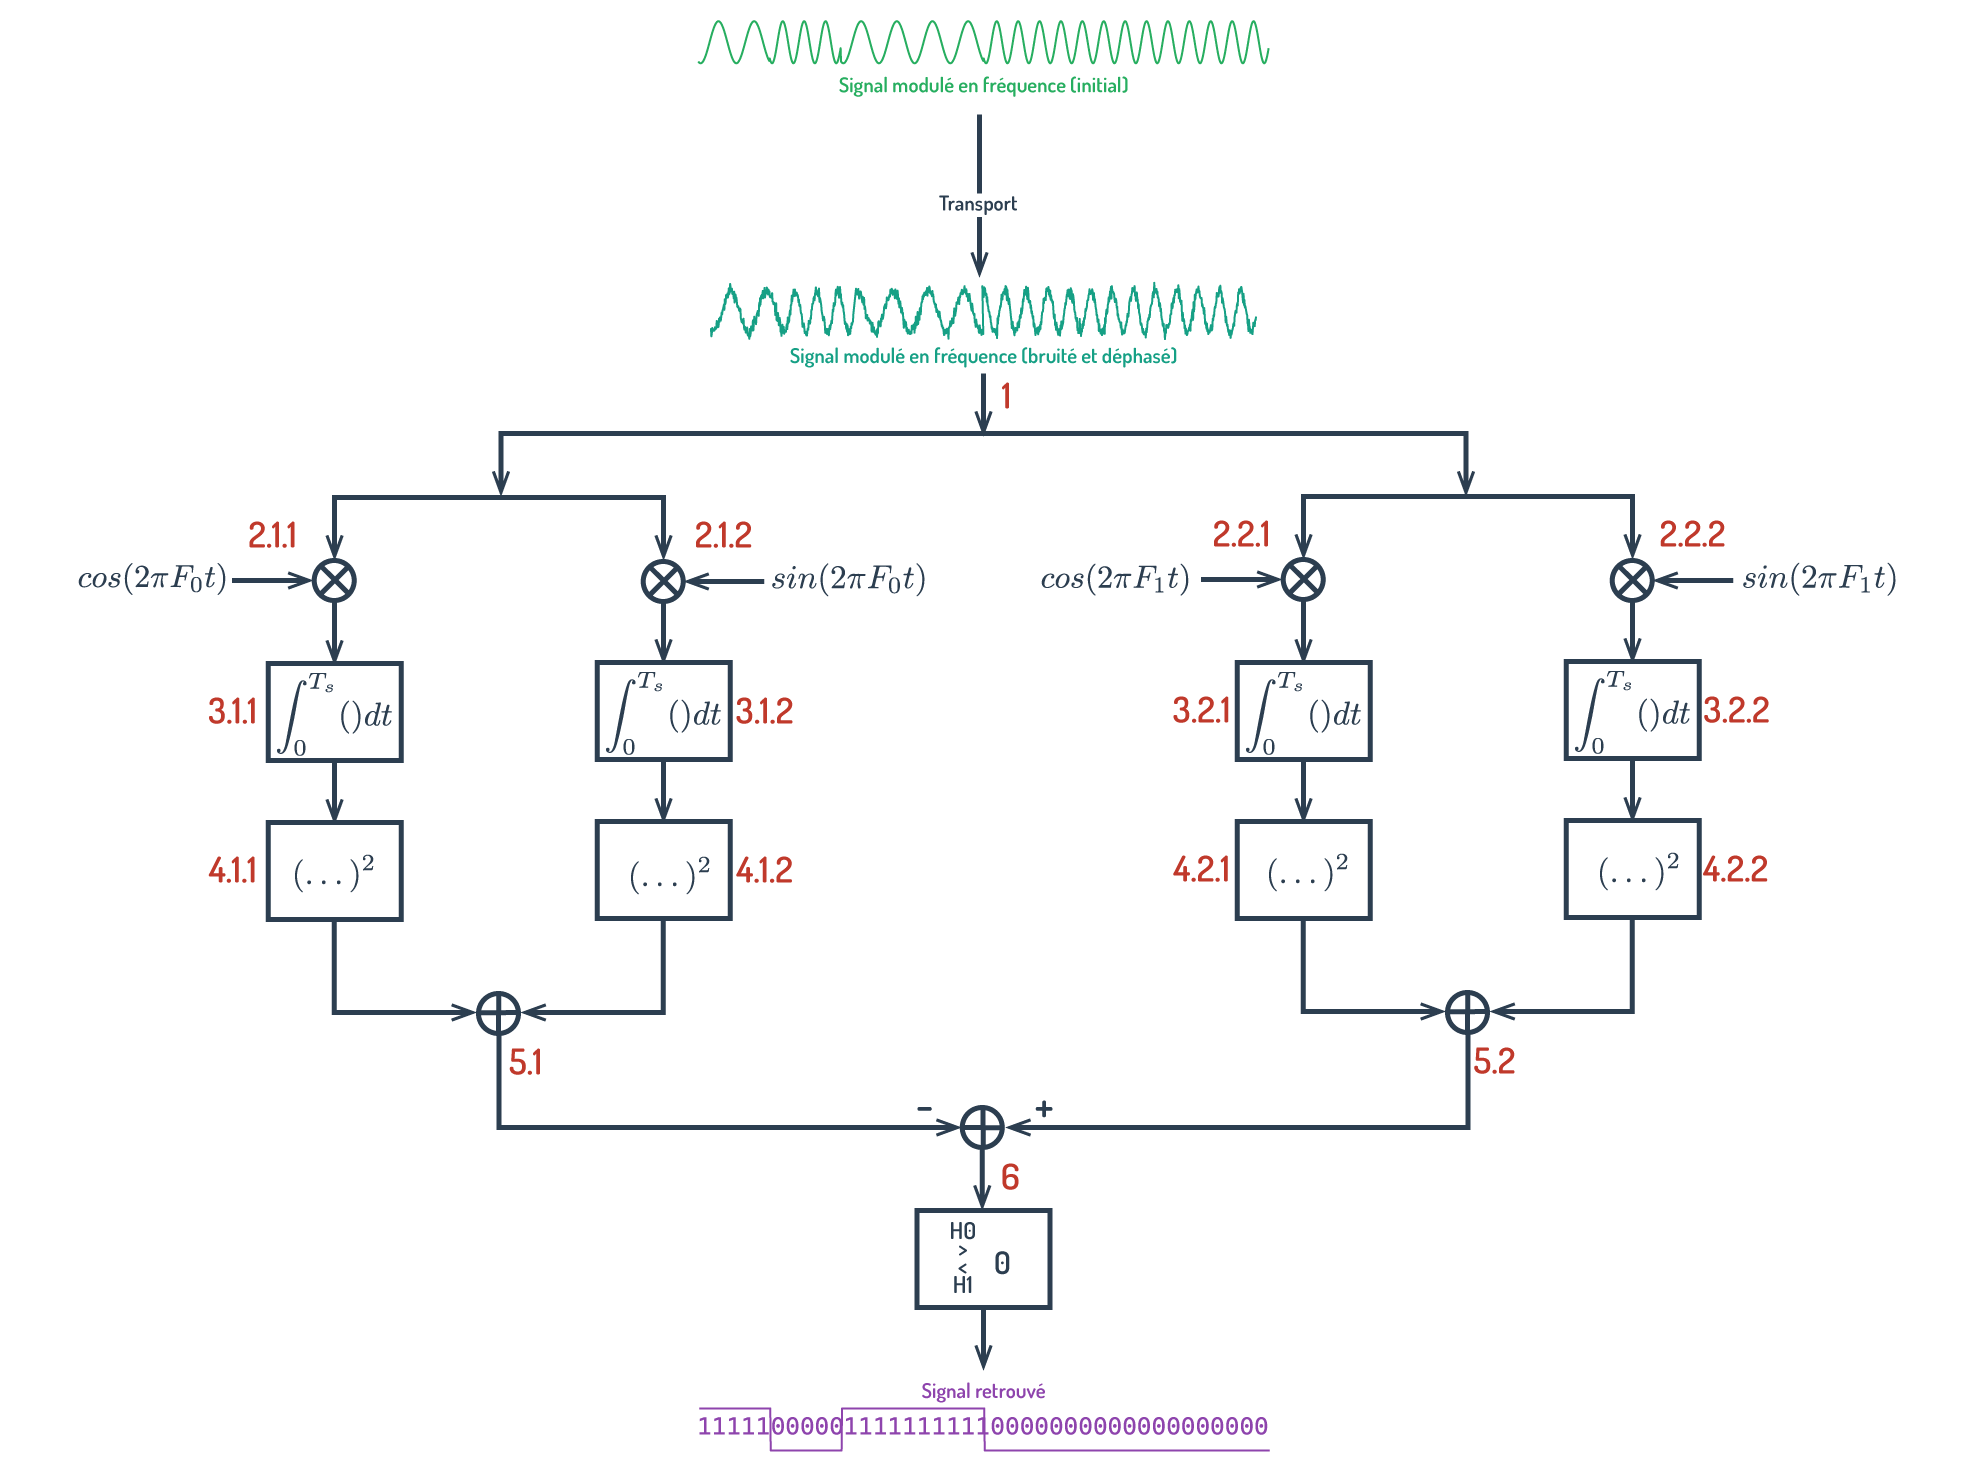
\includegraphics[scale=0.2]{partie-3/sous-partie-2/filtre2.png}
   \caption{Schéma de démodulation FSK avec déphasage.} \label{fig:filtre2}
\end{figure}

Maintenant, si on reprend les calculs, notons $R_i$ le résultat à l'étape $i$.
\[
   R_6 = R_{5.2} - R_{5.1}
\]
Or,
\begin{dinglist}{111}
   \item Si $NRZ = 0$, $R_{5.1} \approx \frac{T_s^2}{4}$ et $R_{5.2} = O(R_{5.1})$, d'où $R_6 = - R_{5.1} < 0$
   \item Si $NRZ = 1$, $R_{5.2} \approx \frac{T_s^2}{4}$ et $R_{5.1} = O(R_{5.2})$, d'où $R_6 = R_{5.2} > 0$
\end{dinglist}

En fait, lors du développement des calculs, le terme $cos(\phi_0-\phi_0')$ disparait à l'aide de la formule $cos^2+sin^2=1$.


\subsubsection{Implémentation du nouveau récepteur}
\begin{lstlisting}[caption=Récepteur V21 avec déphasage, label=code:syn-dephasage]
x0c = x .* cos(2 * pi * F0 * t);
x0s = x .* sin(2 * pi * F0 * t);
x1c = x .* cos(2 * pi * F1 * t);
x1s = x .* sin(2 * pi * F1 * t);

x0c_reshape = reshape(x0c, Ns, Nb_bit);
X0c = sum(x0c_reshape * Te, 1).^2;

x0s_reshape = reshape(x0s, Ns, Nb_bit);
X0s = sum(x0s_reshape * Te, 1).^2;

x1c_reshape = reshape(x1c, Ns, Nb_bit);
X1c = sum(x1c_reshape * Te, 1).^2;

x1s_reshape = reshape(x1s, Ns, Nb_bit);
X1s = sum(x1s_reshape * Te, 1).^2;

X2 = (X1c + X1s) - (X0c + X0s);
Donnee_retrouve_3 = X2 > 0;

Nb_erreur_3 = sum(Donnee ~= Donnee_retrouve_3);
taux_erreur_3 = Nb_erreur_3 / Nb_bit;
\end{lstlisting}

On retrouve alors un \textcolor{Red}{taux d'erreur de 0\%}.